\section{Modelling the Game}
\label{sec:model}

% what this section talks about
%   - graph of objects and relations
%   - what each model object represents and is
%   - difficulties developing the model
%   - model: sector, game, entity, ship, plan, goal, ship action, ship class, ship configuration, weapon, system, weapon slot, system slot, fleet, Formation, client state
% what is a game model
% early on
% 

The model that makes up the game consists of the internal representation of the various game entities, such as ships and planets, as well as the business logic that is used to manage and control them and the relationships between them. During the alpha phase, this model was rather simple as it only existed to store the locations of the entities. As development progressed, it grew in complexity and feature completeness. Currently there are complex models for the fleets of ships, and the map of planets and spacelanes.\sidenote{Spacelanes are connections between some planets that allow ships travelling along or nearby them to move more quickly. See Section~\ref{sec:pathfinding} for complete details.} This section will describe and discuss these models and the reasonings behind their design.

\begin{margintable}
    \begin{tabular}{p{4em} p{11em}}
    \toprule
    \emph{Field} & \emph{Description} \\
    \midrule

    Name & Sector name \\
    Size & Sector dimensions \\
    Spawn points & List of locations where different players' fleets are spawned \\
    Planets & List of planets in the sector \\
    Spacelanes & List of spacelanes that connect the planets \\

    \bottomrule
    \end{tabular}
    \vspace{1em}
    \caption{Fields of the Sector model}
    \label{tab:sector-fields}
\end{margintable}

The different game maps are known as sectors. A sector models all of the planets in a battle, how they are connected with spacelanes, and where the different spawn points are located. The actual fields that make up the sector model are shown in Table~\ref{tab:sector-fields}. Sectors have different sizes because it allows the players to customise the play time required for a battle to some degree. Choosing a larger sectors will typically result in a longer battle than smaller ones. The specification has a requirement for short battles, but it is good to add some flexibility to allow players the freedom to decide how to enjoy the game. It could have been possible to have static spawn points that are enforced for all sectors, for example spawning players in the corners of the sector so that they are as far apart as possible. However, the actual design has per sector spawn points so that the spawn points can be customised to be as fair as possible relative to the layout of the planets within the sector. This decision was made to make the game as balanced as possible to maximise the enjoyment of all players.

% The sector specifies which planets are includes as well as which planets are connected by space lanes as shown in Figure \ref{fig:model:sectorRelation}

% \begin{marginfigure}
% 	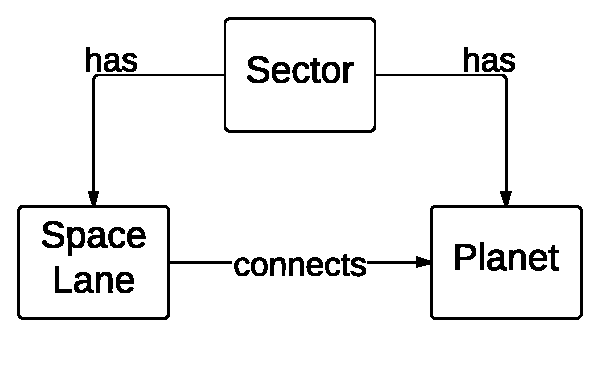
\includegraphics{res/model/sector.pdf}
% 	\caption{relationship between setor, planet, and space lanes}
% 	\label{fig:model:sectorRelation}
% \end{marginfigure}

\begin{margintable}
    \begin{tabular}{p{4em} p{11em}}
    \toprule
    \emph{Field} & \emph{Description} \\
    \midrule
    Name & Planet name \\
    Ecotype & Type of planet, e.g. star, ocean, or desert \\
    Location & Location of planet within the sector \\
    Resources & Quantity of resources generated by the planet if captured \\
    Capture status & Current owner of the planet, if any, and by how much they have captured it \\
    \bottomrule
    \end{tabular}
    \vspace{1em}
    \caption{Fields of the Planet model}
    \label{tab:planet-fields}
\end{margintable}

The list of planets that make up the sector are specified using the planetary model. Planets are modelled in such a way as to have a number of different fields that make the planet unique. Table~\ref{tab:planet-fields} gives a breakdown of the properties that comprise the model of a planet. Just like sectors, planets have a nickname to allow players to easily reference a specific planet instead of having to use location information or numerical identifiers. One of the most interesting pieces of the planetary model is the \emph{ecotype}. The ecotype of a planet specifies the type of ecological system that the planet represents, for example the ocean ecotype is used for planets that are almost entirely covered by water. This ecotype has a big effect on the planet because it determines the quantities of the different resources found in the planet.\sidenote{The use of resources is laid out in detail in Section~\ref{sec:resources}} This is because, for example, some ecotypes will have a greater proportion of metal (e.g.\ the metal ecotype). However, the quantity of resources stored by a planet is actually represented by a separate field instead of being statically determined by the ecotype. This was done to make it possible to add some more variety to the different planets. For example, it could be possible to use a random number generator to set the quantities of resources in a planet within the range specified by its ecotype. Currently all resource quantities are specified statically, but this potential enhancement would add some variables to the battles to keep the game interesting for regular players.

% TODO fix margin diagrams, all appearing below the page (invisible)
% \begin{marginfigure}
% 	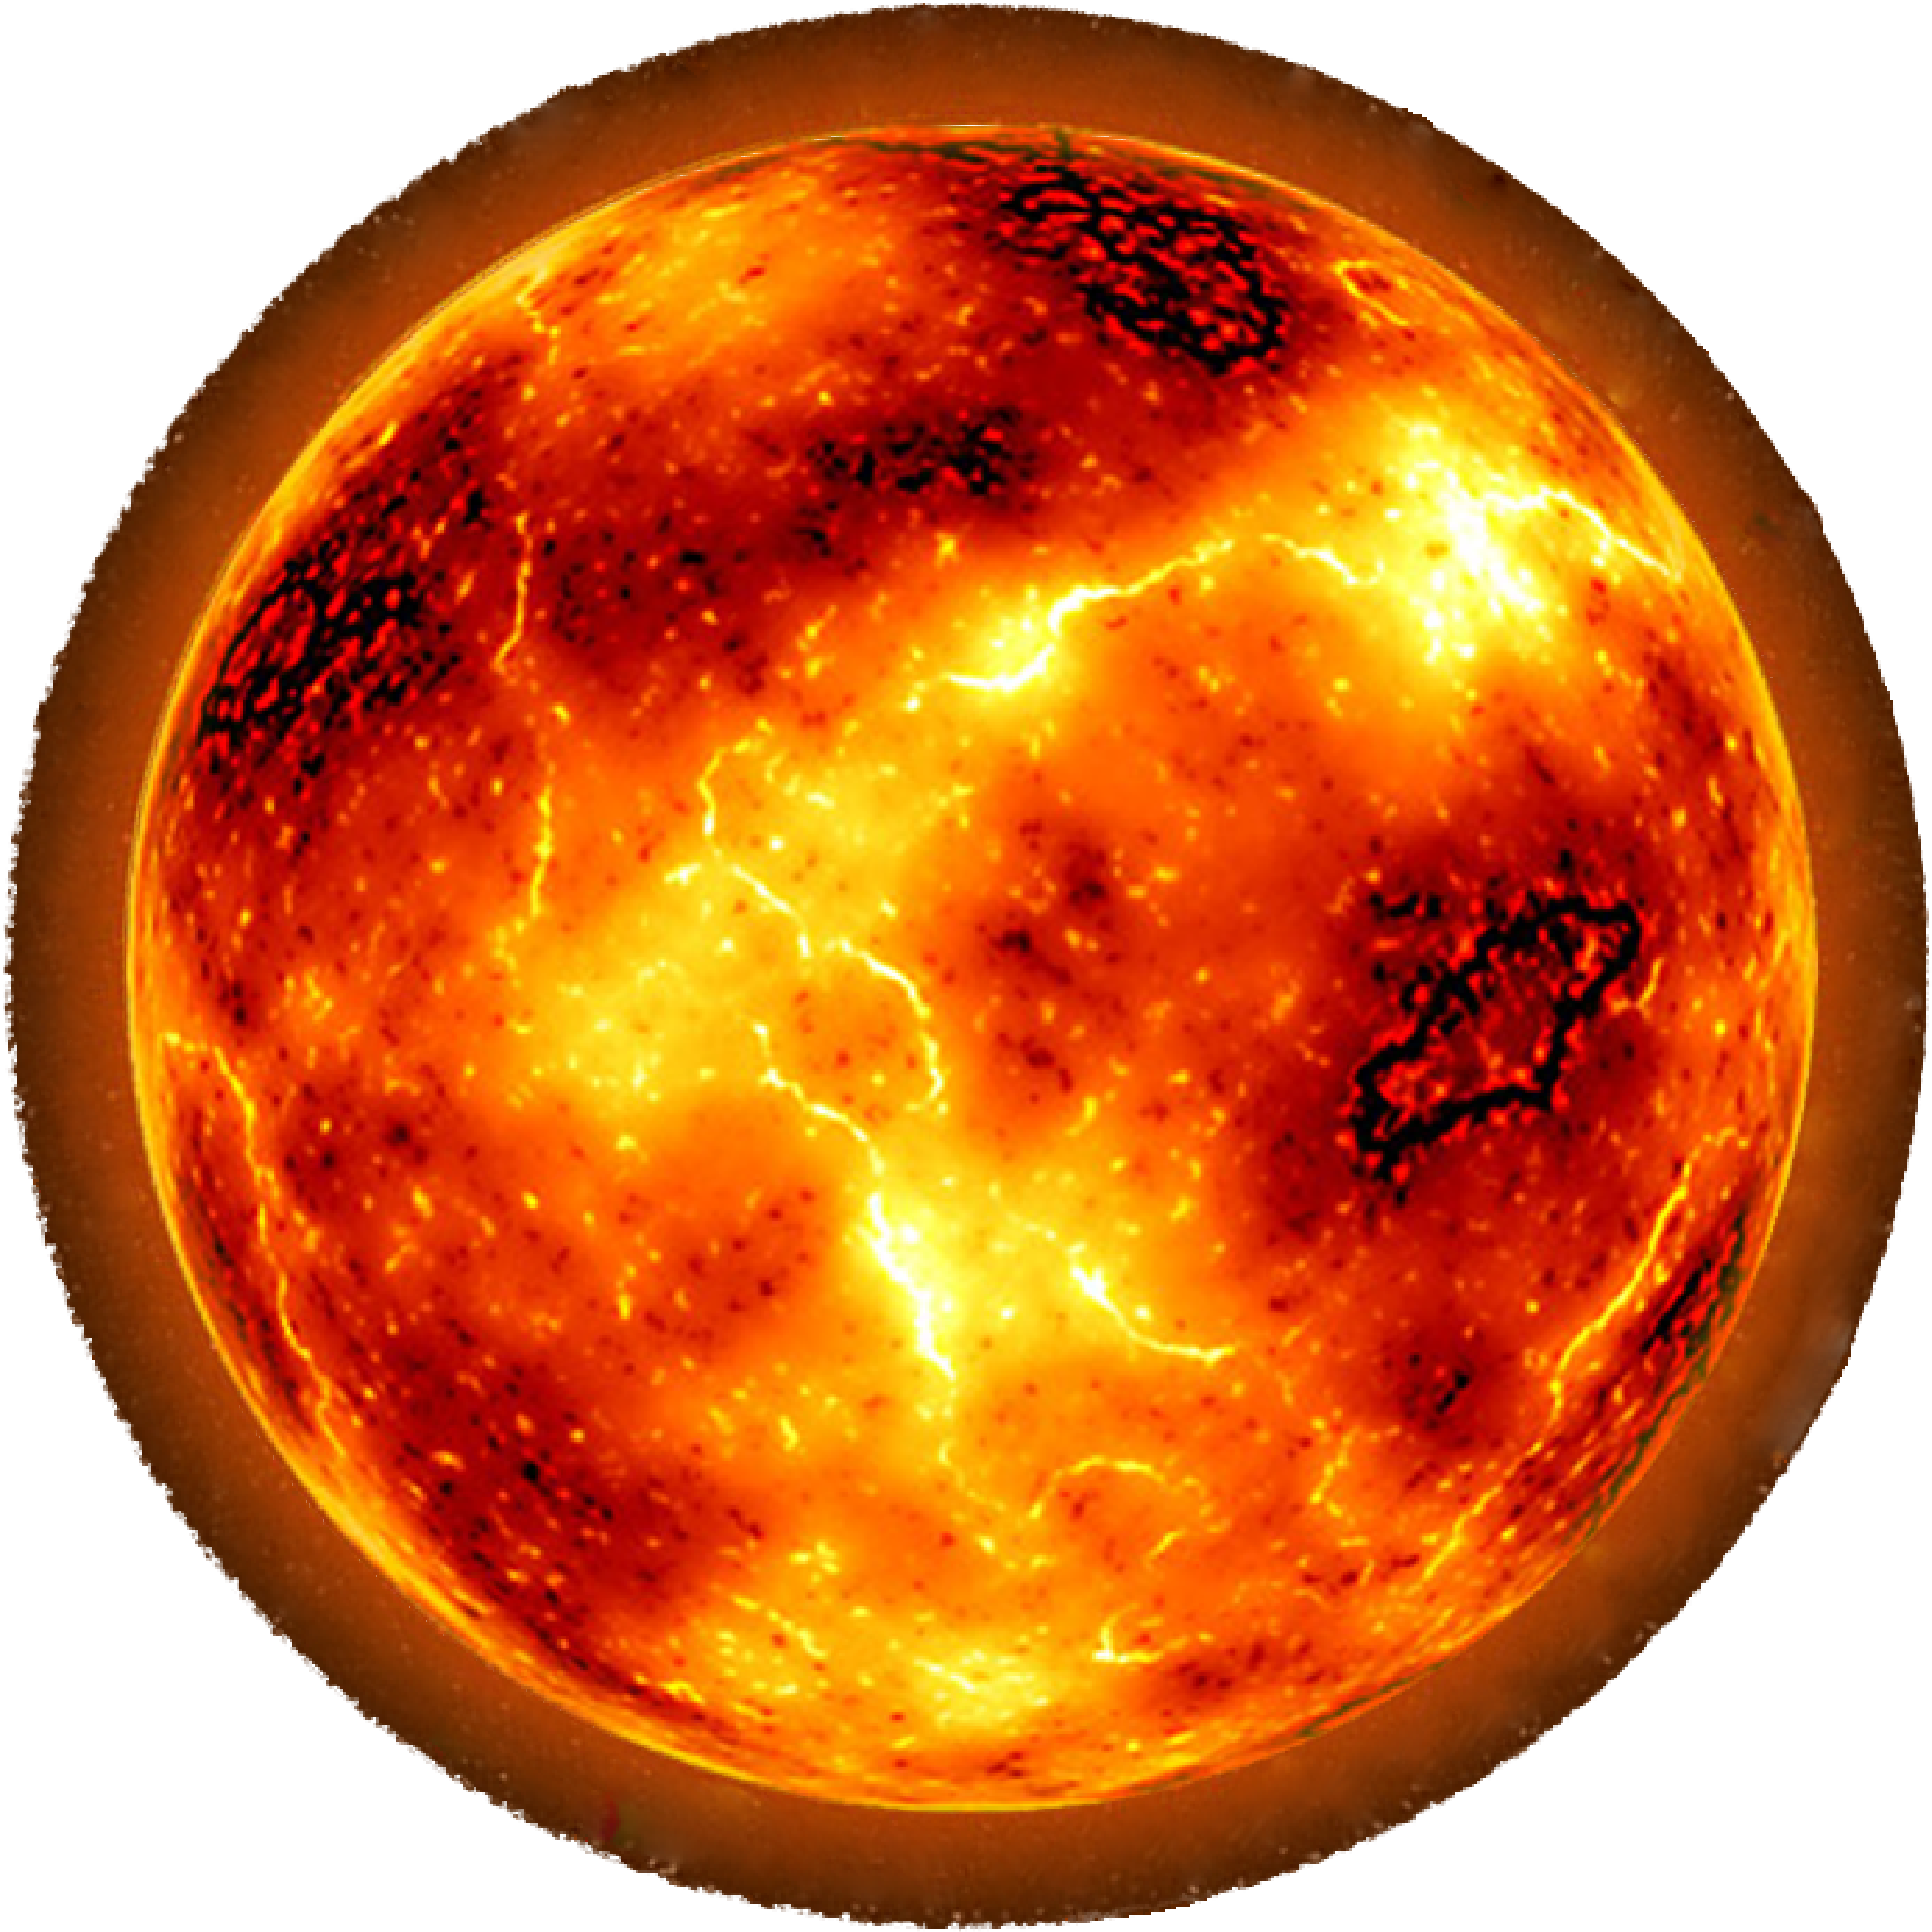
\includegraphics{res/planets/star.png}
% 	\caption{ecotype: star}
% 	\label{fig:model:starPlanet}
% \end{marginfigure}
% 
% \begin{marginfigure}
% 	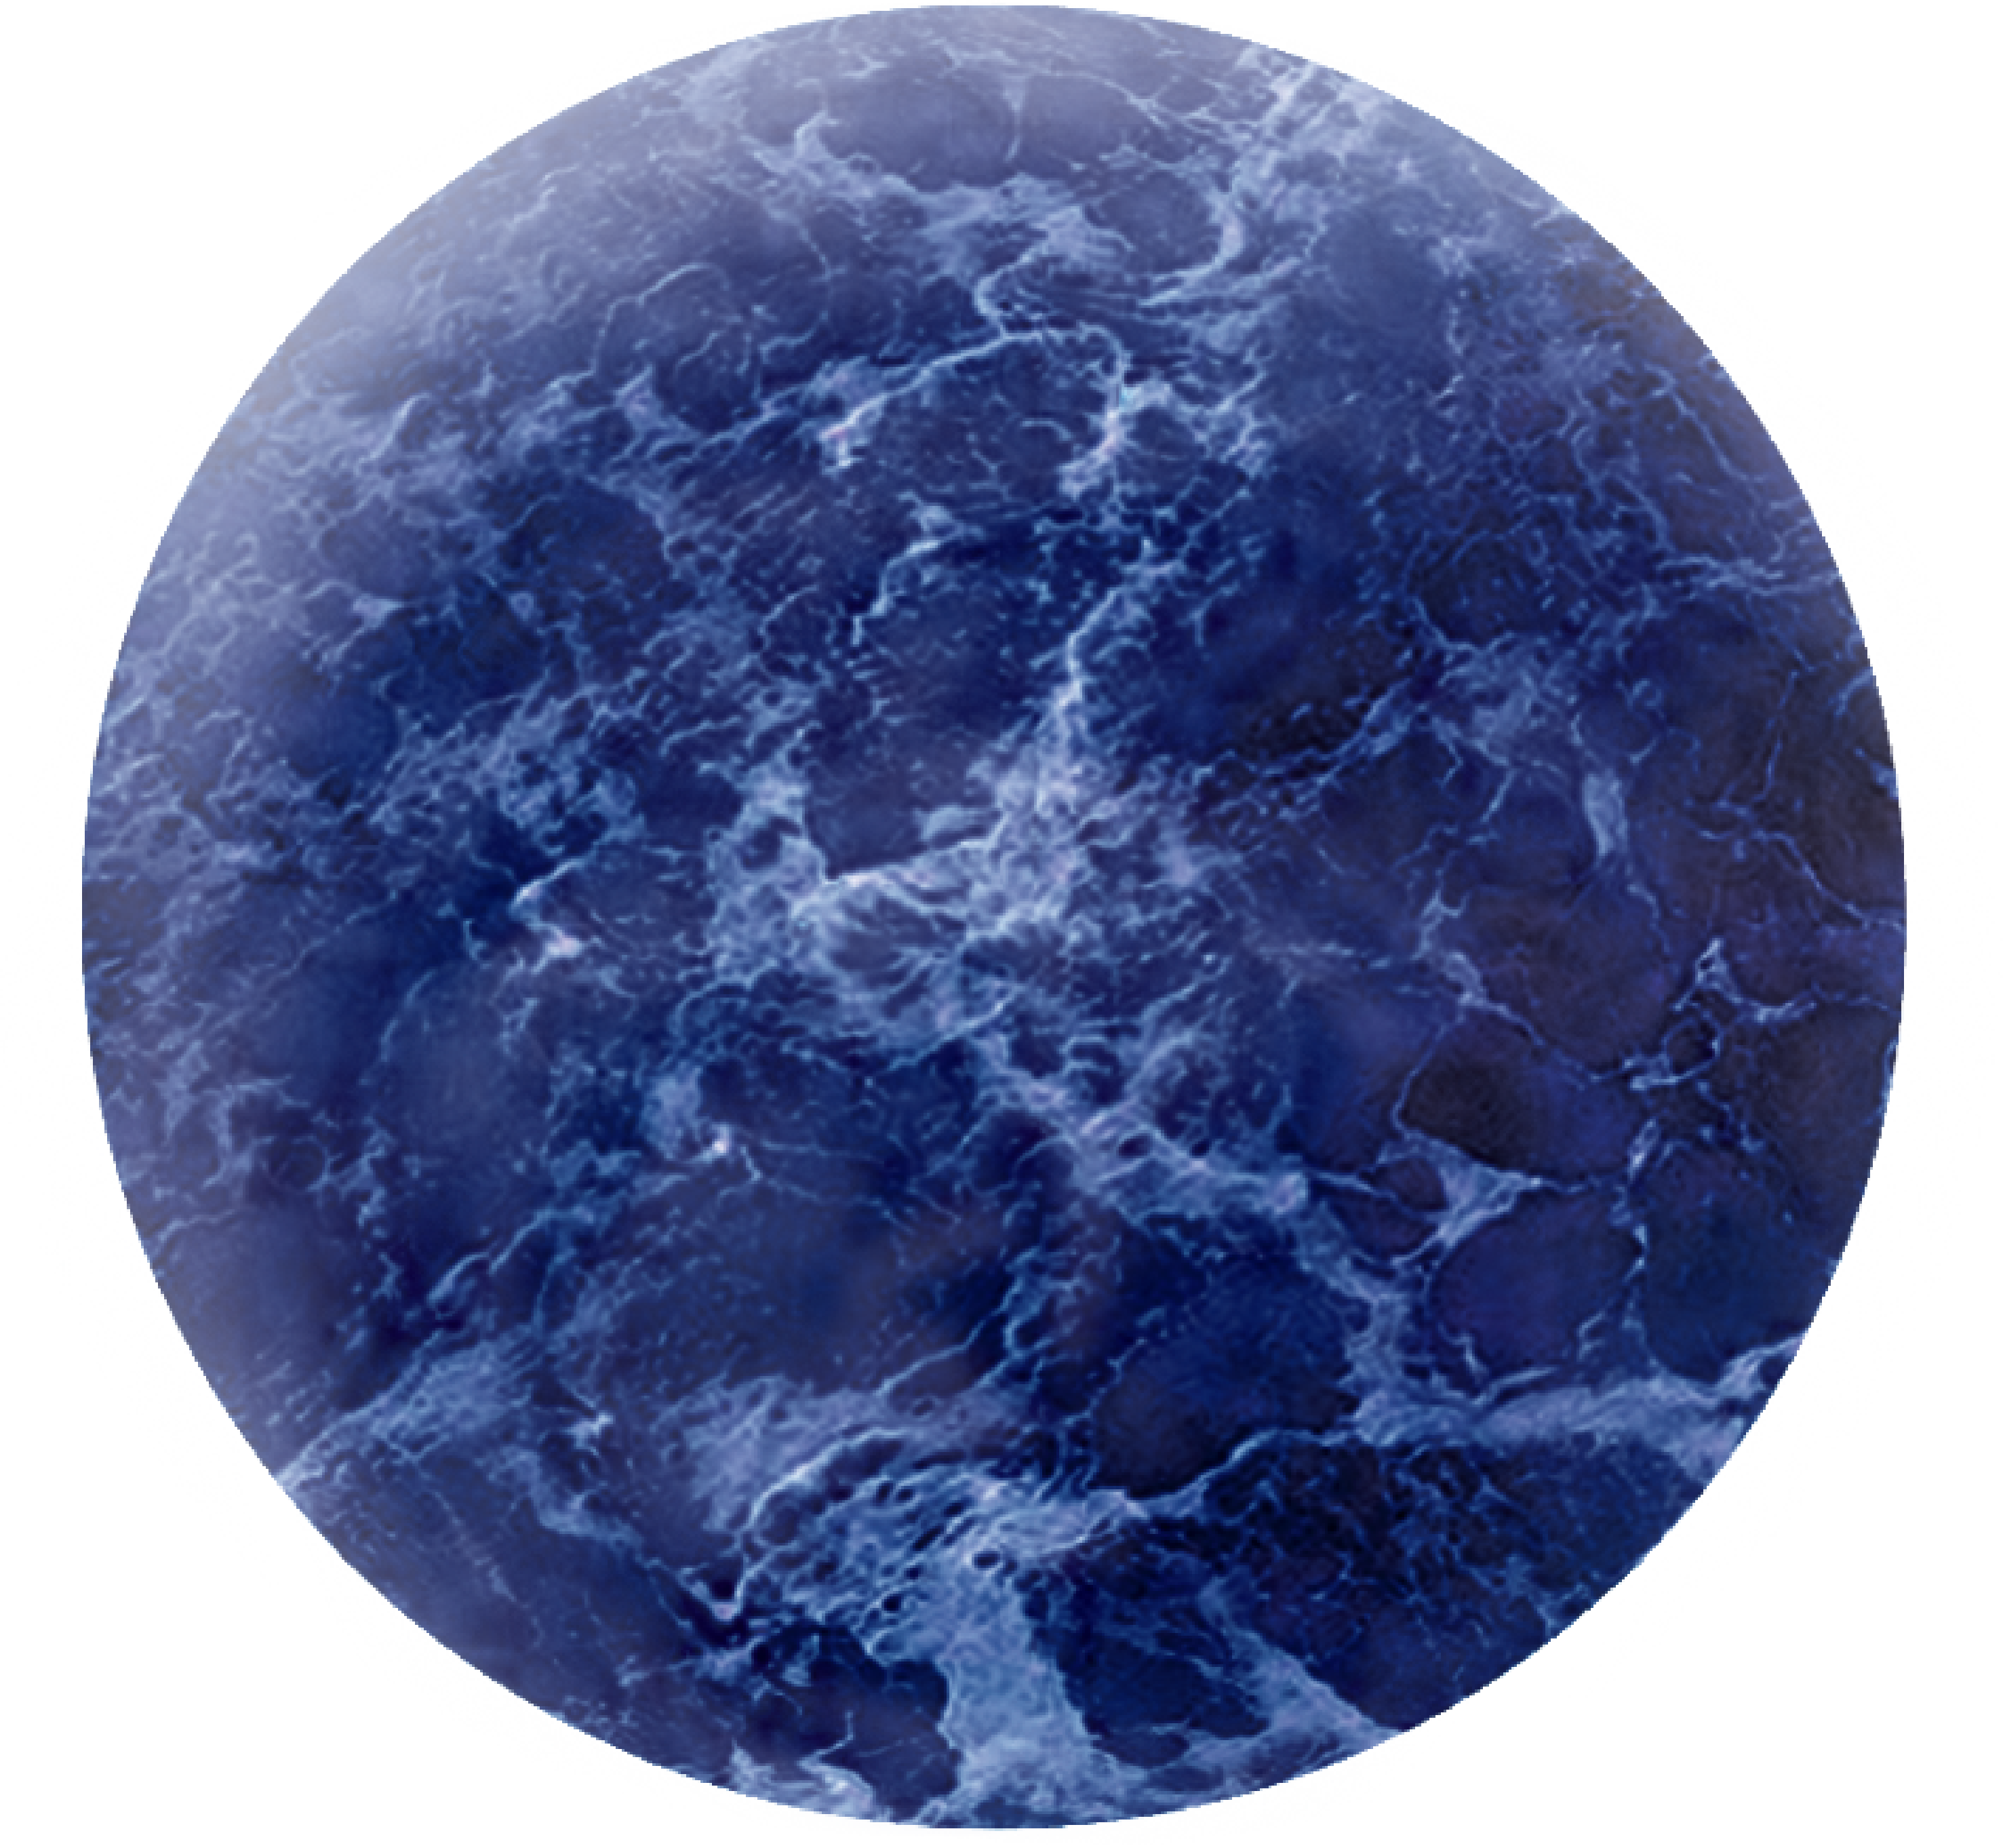
\includegraphics{res/planets/OceanPlanet.png}
% 	\caption{ecotype: ocean}
% 	\label{fig:model:oceanPlanet}
% \end{marginfigure}
% 
% \begin{marginfigure}
% 	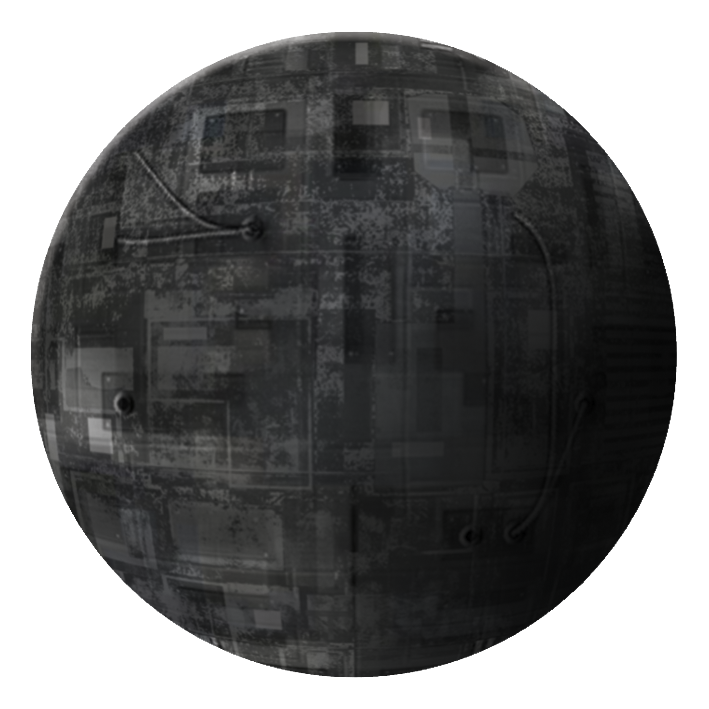
\includegraphics{res/planets/metal-planet.png}
% 	\caption{ecotype: metal}
% 	\label{fig:model:metalPlanet}
% \end{marginfigure}

% ship
The ship part of the model is actually broken down into 3 key concepts: Ship, Ship Configuration and Ship Class.
The Ship Class represents the the hull of the ship, its size, number of weapon sots etc. Every ship in the game will have exactly one ship class. The Ship Configuration specifies which weapons and systems go in which slots. Figure \ref{fig:model:shipRelation} demonstrates this relation.
This distinction between Ship, Ship Configuration and Ship Class was a revised addition, because it allowed multiple ships to belong to the same class as well as being able to save the ship configuration to disk, whilst it wouldn't make sense to save a ship to disk since it only exists in that instance of the game.

% ship class
The ship class is a container that is treated as the ship's hull, but in fast it provides more information than just that, it also provides meta-data about the image being used as the ship's hull.
The image being used for the ship's hull has no meta-data attached to it, so this must be specified somewhere, and it is, in the ship class.
The reason the image needs this meta-data is because properties such as centre of rotation cannot be determined. 
They are intrinsically linked to the style of ship. 
For example take 2 images used for ship's hulls, they have identical dimensions but the first one has engines at the front of the ship so you would want the centre of rotation much closer to the front than the second one. 
Table \ref{tab:model:shipClassFields} gives a detailed description of the ship class properties.

\begin{marginfigure}
	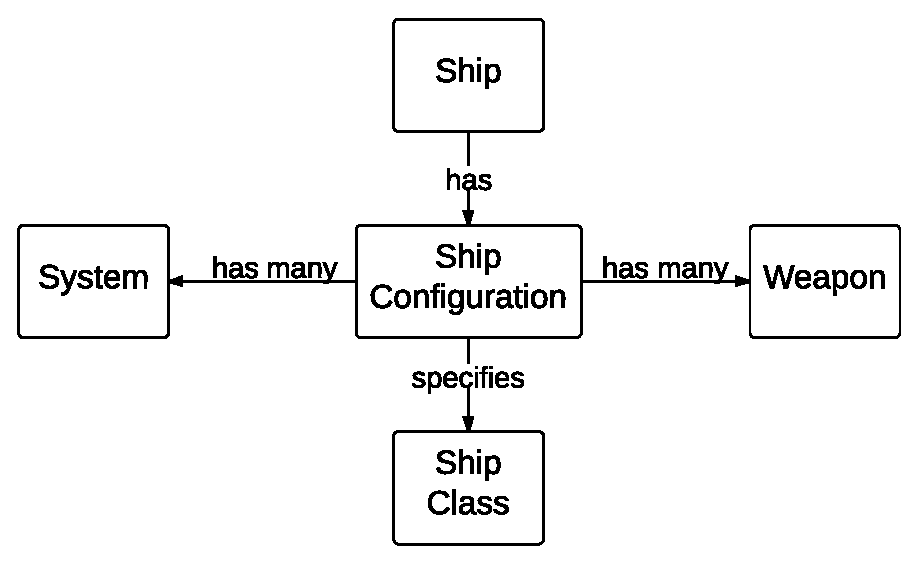
\includegraphics{res/model/ship.pdf}
	\caption{ship layout}
	\label{fig:model:shipRelation}
\end{marginfigure}

\begin{margintable}
    \begin{tabular}{p{4em} p{11em}}
    \toprule
    \emph{Fields} & \emph{Description} \\
    \midrule
    centre of rotation & point on the ship class where it rotates when turning \\
    speed & maximum speed of this hull \\
    health & health of the hull \\
    weapon slots & specifies where the weapon slots are on the hull and what type they are \\
    system slots & specifies where the system slots are on the hull \\
    name & name of the hull, used by player \\
    cost & cost of adding a ship with this hull to the fleet \\
    \bottomrule
    \end{tabular}
    	\vspace{1em}
	\caption{properties of ship class}
	\label{tab:model:shipClassFields}
\end{margintable}


% ship, ship configuration, ship class, weapons, system
